
\section{Węzły torusowe}
\index{węzeł!torusowy|(}%

W tej sekcji przyjrzymy się węzłom o~specjalnym ułożeniu w~przestrzeni $\R^3$.
Do ich określenia potrzebny jest torus trywialny, powierzchnia otrzymana przez obrót okręgu $(x-2)^2 + y^2 = 1$ wokół osi $y$.
Można go także uzyskać przez sklejenie podstaw walca tak, by go przy tym nie zapętlić.
Oczywiście istnieją też nietrywialne torusy, jak rurowe otoczenie trójlistnika.

Sploty torusowe wprowadza króciutko Kawauchi \cite[s. 26-27]{kawauchi96}.
% TODO: rozdział Standard examples powinien zostać przetworzony w odwołania takie jak to wyżej w każdej naszej sekcji, nie tylko Węzły torusowe

\begin{definition}[splot torusowy]
    Splot, który leży na powierzchni trywialnego torusa, nazywamy torusowym.
\end{definition}

Na walcu $S^2 \times [0,1]$, którego podstawa leży w~płaszczyźnie $xy$, rozpatrzmy $r$ skierowanych odcinkach (dla $k = 0, 1, \ldots, r - 1$) o~końcach w~punktach
\begin{align*}
    \left(\cos \frac{2k \pi}{r}, \sin \frac{2k\pi}{r}, 0 \right), \quad
    \left(\cos \frac{2k \pi}{r}, \sin \frac{2k\pi}{r}, 1 \right).
\end{align*}
Przekręćmy górną podstawę walca wokół osi $z$ o~skierowany kąt $2\pi q / r$ oraz utożsammy ze sobą pary punktów $(x, y, 0) \sim (x, y, 1)$,
Uzyskaliśmy splot torusowy $T_{q, r}$: okrąża on $q$ razy rdzeń torusa i~$p$ razy jego oś symetrii obrotowej.
Węzeł $T_{p, q}$ posiada następującą parametryzację:
\[
    x = (2+\cos q \phi) \cos p \phi, \quad
    y = (2+\cos q \phi) \sin p \phi, \quad
    z = - \sin q \phi, \quad
    0 \le \phi \le 2\pi.
\]
Poniżej przedstawiamy trzy węzły torusowe.

\begin{figure}[H]
    \begin{minipage}[b]{.3\linewidth}
        \centering
        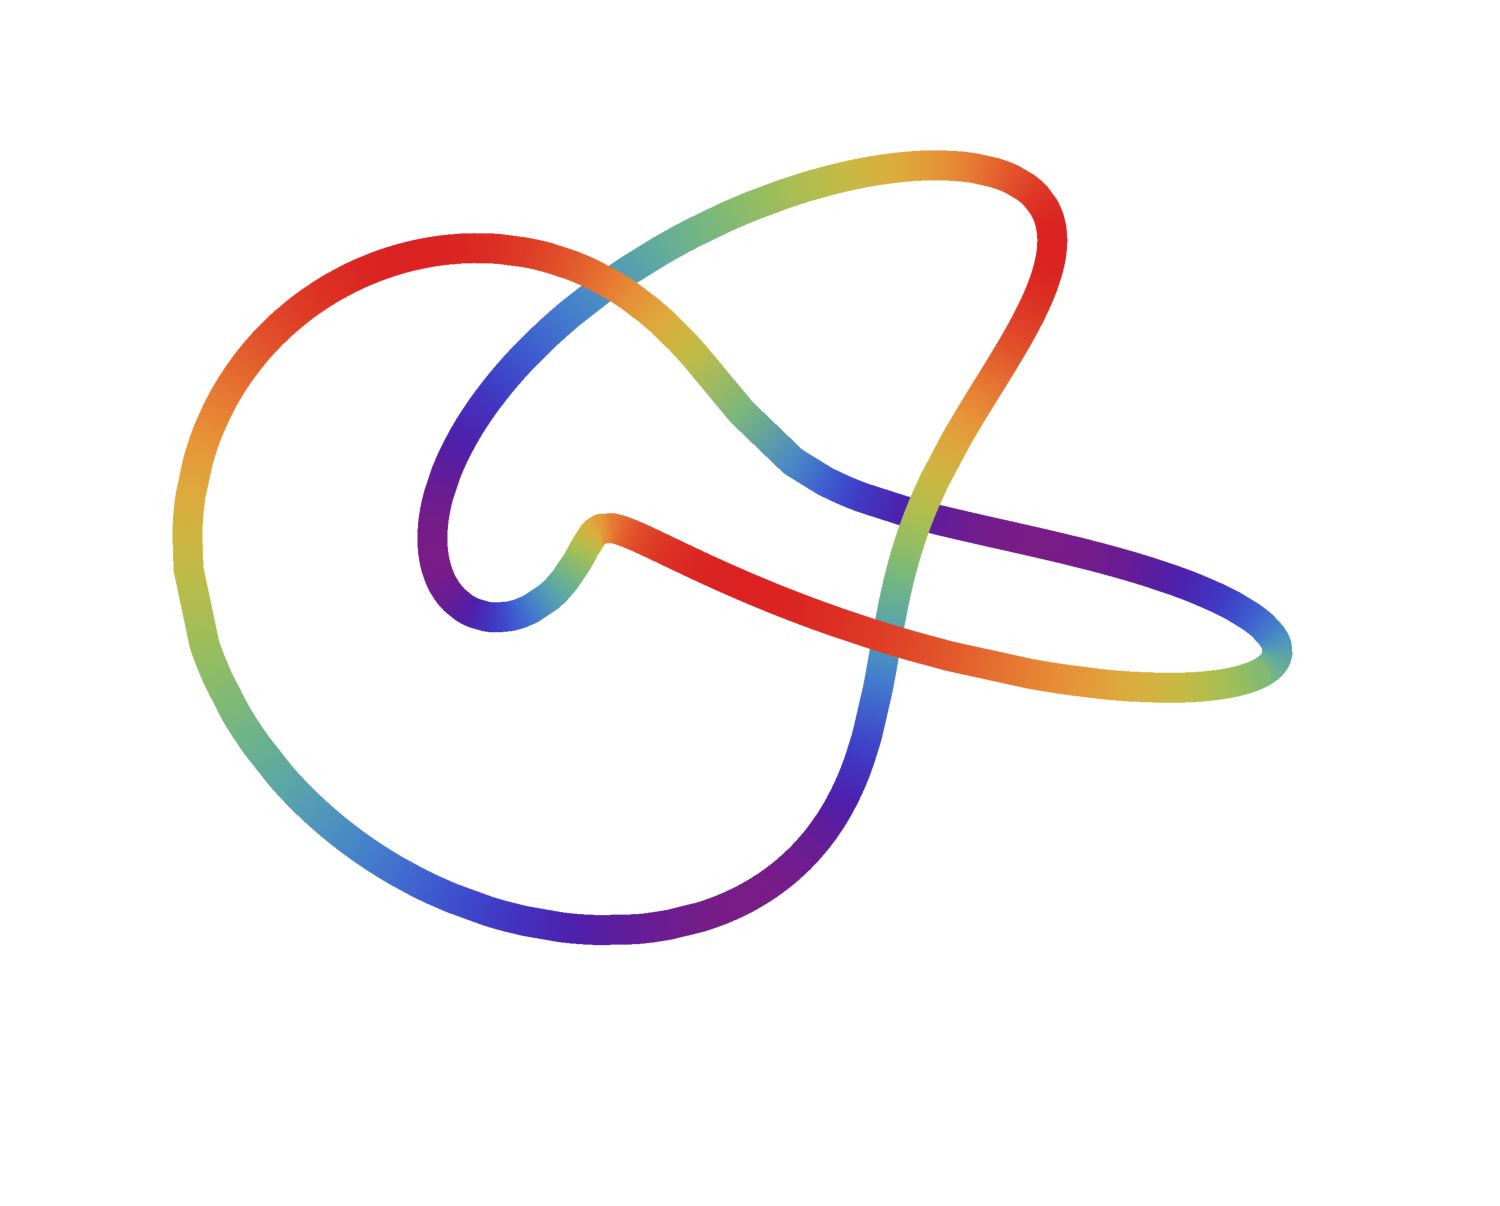
\includegraphics[width=\linewidth]{../data/torus-p2-q3.pdf}
        \subcaption{trójlistnik: $p = 2, q = 3$}
    \end{minipage}
    \begin{minipage}[b]{.3\linewidth}
        \centering
        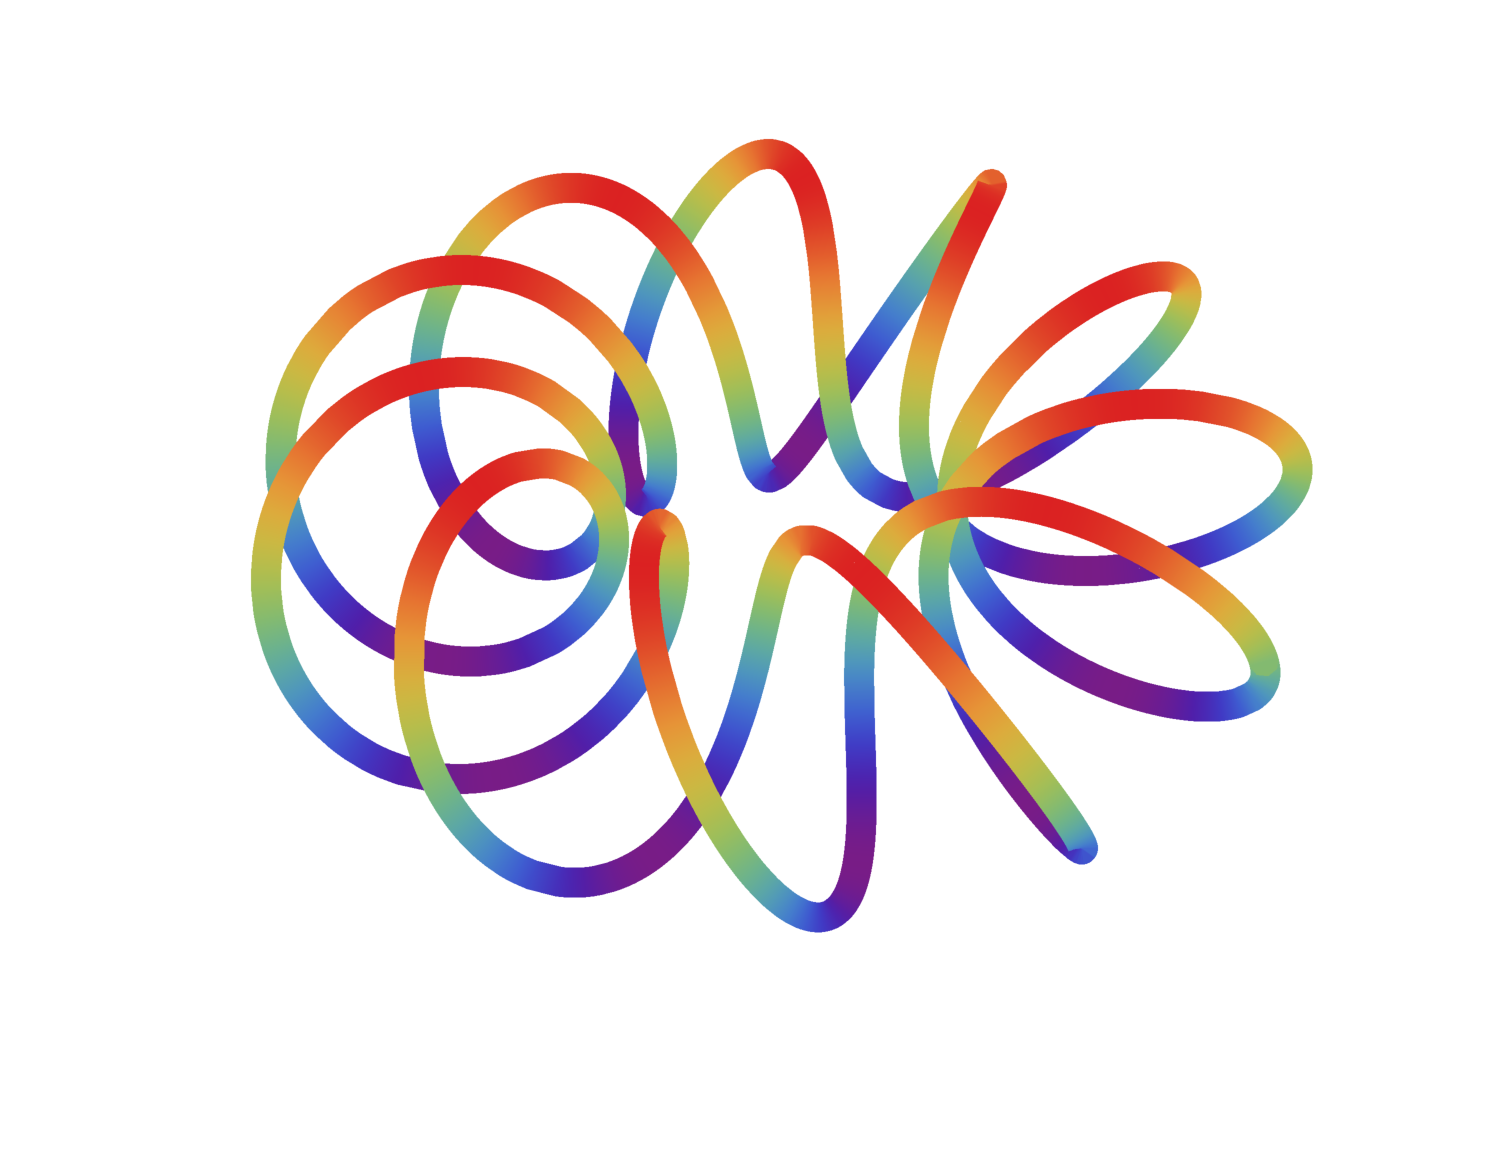
\includegraphics[width=\linewidth]{../data/torus-p2-q11.pdf}
        \subcaption{$p = 2, q = 11$}
    \end{minipage}
    \begin{minipage}[b]{.3\linewidth}
        \centering
        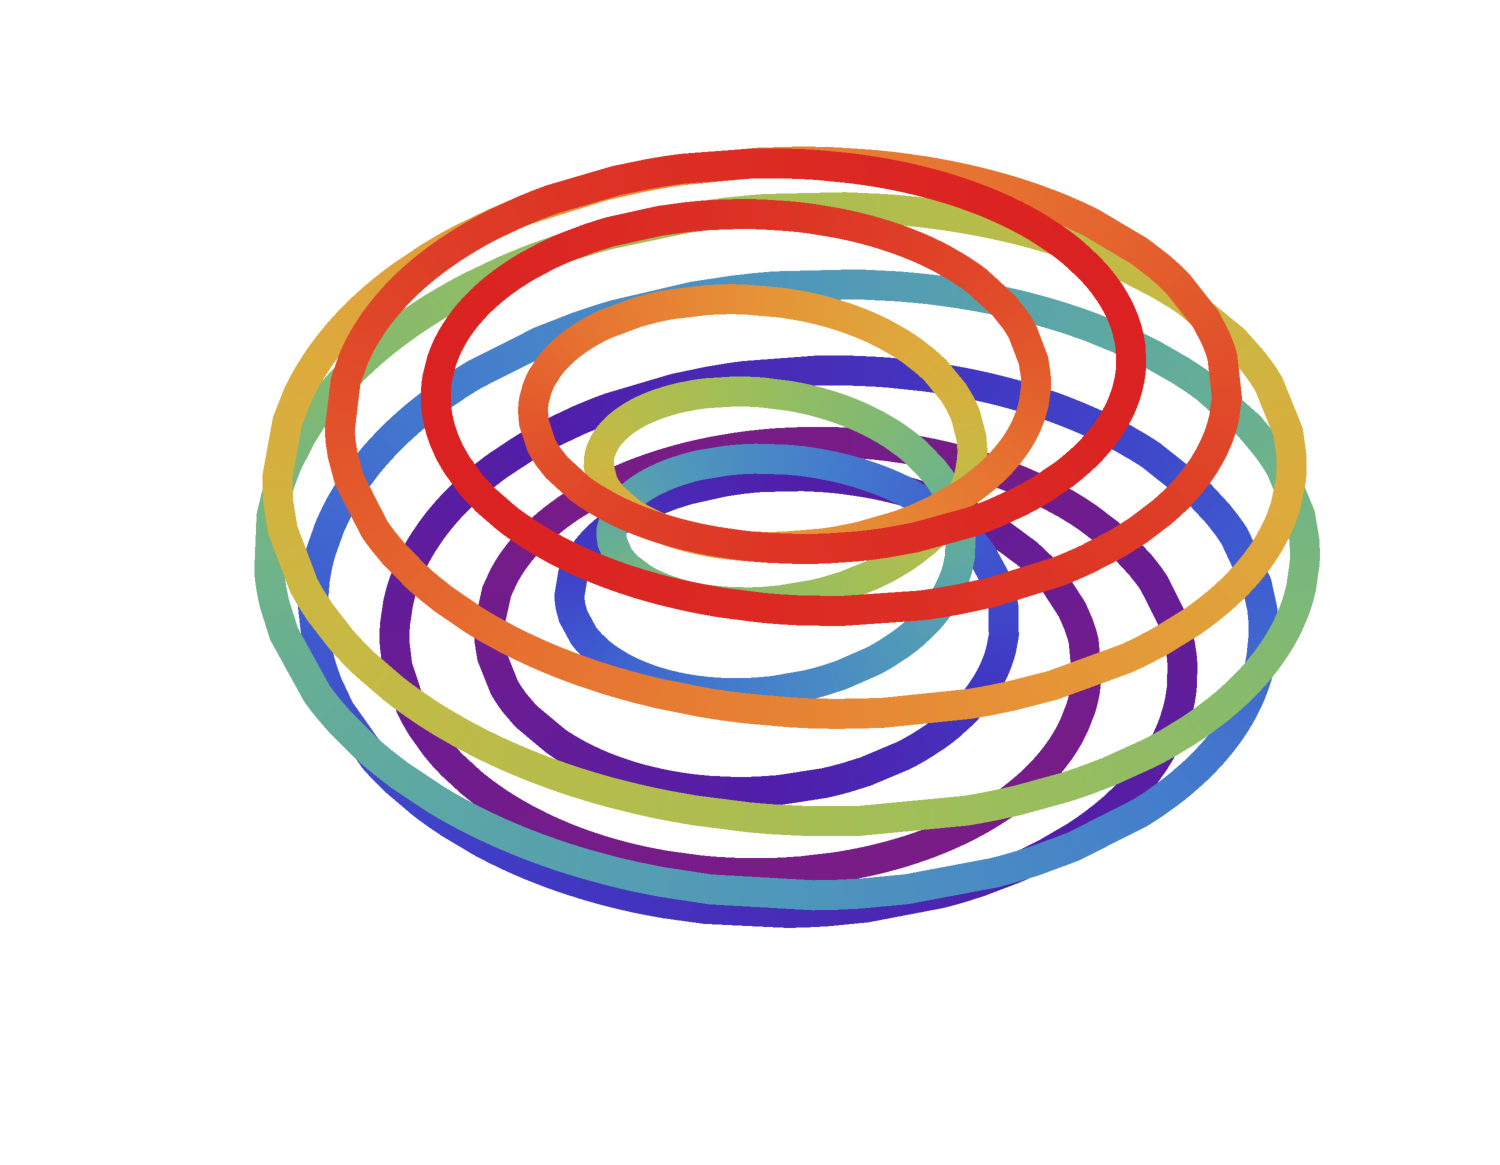
\includegraphics[width=\linewidth]{../data/torus-p11-q2.pdf}
        \subcaption{$p = 11, q = 2$}
    \end{minipage}
\end{figure}

Murasugi \cite[s. 135]{murasugi96} pisze, że będzie nazywać okrąg leżący na powierzchni torusa $T_{0, 0}$ (chociaż według naszej parametryzacji to byłby punkt), natomiast (do napisania!).
% todo: http://www.matematyka.wroc.pl/leksykonmatematyczny/torus
% p = 1; q = 0; pp = 3; qq = 7; ParametricPlot3D[{{Cos[ 2 Pi p t] (2 + Cos[2 Pi q t]), (2 + Cos[2 Pi q t]) Sin[ 2 Pi p t], -Sin[2 Pi q t]}, {Cos[ 2 Pi pp t] (2 + Cos[2 Pi qq t]), (2 + Cos[2 Pi qq t]) Sin[ 2 Pi pp t], -Sin[2 Pi qq t]}}, {t, 0, 1}, ColorFunction -> "Rainbow", PlotStyle -> Thickness[0.02], Boxed -> False, Axes -> False]
% 1, 0 czy 0, 1? Wydaje mi się, że my mamy to na odwrót
% Węzeł $T_{0, 0}$ leży na powierzchni torusa i~jest ściągalny do punktu, zaś $T_{1, 0}$ to nawinięta toroidalnie pętla.

%Węzeł ten leży na torusie $(r - 2)^2 + z^2 = 1$.
% p = 5;
% q = 3;
% ParametricPlot3D[
% {
% Cos [2 Pi p t] (2 + Cos[2 Pi q t]),
% (2 + Cos[2 Pi q t]) Sin[2 Pi p t],
% -Sin[2 Pi q t]},
% {t, 0, 1},
% ColorFunction -> "Rainbow",
% PlotStyle -> Thickness[0.02],
% Boxed -> False,
% Axes -> False
% ]

Okazuje się, że innych obiektów już nie ma.

\begin{proposition}
    Niech $K$ będzie splotem torusowym takim, że żadne z jego ogniw nie jest niewęzłem, czyli postaci $T_{1, 0}$.
    % T 1,0 czy T 0,1?
    Wtedy $K = T_{p, q}$ dla pewnych całkowitch $p, q$.
\end{proposition}

\begin{proposition}
    Niech $d$ będzie największym wspólnym dzielnikiem liczb całkowitych $p, q$.
    Wtedy węzeł torusowy $T_{p, q}$ posiada dokładnie $d$ ogniw.
\end{proposition}

Siedem węzłów z tabeli na końcu książki to węzły torusowe.
Są to niewęzeł, $3_1 = T_{3,2}$, $5_1 = T_{5,2}$, $7_1 = T_{7,2}$, $8_{19} = T_{4,3}$, $9_1 = T_{9,2}$ oraz $10_{124} = T_{5, 3}$.

\begin{proposition}
    Niech $p, q$ będą względnie pierwszymi liczbami takimi, że $|p|, |q| \ge 2$.
    Wtedy splot $T_{p, q}$ oraz splot do niego odwrotny, $T_{-p, -q}$, są tego samego typu.
\end{proposition}

Sploty $T_{p, q}$ oraz $T_{q, p}$ również są równoważne.
Murasugi prezentuje w~swojej książce \cite{murasugi96} przyjemny dowód opierający się na następującym lemacie:

\begin{lemma}
    Sfera $S^3$ powstaje z~powierzchni dwóch węzłów trywialnych z~wnętrzem ($D^2 \times S^1$) przez wzajemne sklejenie południka i~równoleżnika z~równoleżnikiem i~południkiem.
\end{lemma}

Węzły torusowe są pierwsze, czego dowód można znaleźć u Burdego, Zieschanga \cite[s. 95]{burde14}, chociaż nie wiem, kto pierwszy to zauważył.

\begin{proposition}
\label{prp:torus_nontrivial_center}
    Niech $K$ będzie nietrywialnym węzłem, którego grupa podstawowa $\pi$ ma nietrywialne centrum.
    Wtedy $K$ jest węzłem torusowym.
    % Kawauchi: The torus knots are characterized as the only knots whose groups have non-trivial centers (cf. Corollary 6.3.6).
\end{proposition}

\begin{proof}
\index[persons]{Aumann, Robert}
% https://mathscinet.ams.org/mathscinet-getitem?mr=96236
\index[persons]{Burde, Gerhard}%
\index[persons]{Murasugi, Kunio}%
\index[persons]{Neuwirth, Lee}%
\index[persons]{Nielsen, Jakob}%
\index[persons]{Stallings, John}%
\index[persons]{Zieschang, Heiner}%
    Najpierw pokazali to Murasugi \cite{murasugi61}, Neuwirth \cite{neuwirth61} przy dodatkowym założeniu, że węzeł $K$ jest alternujący,
    wkrótce po tym Burde, Zieschang znaleźli dowód w ogólnym przypadku \cite{zieschang66}.
    Ich dowód korzysta z wyników Neuwirtha (komutant grupy $\pi$ jest skończenie generowany), Stallingsa (dopełnienie $X$ tubularnego otoczenia $K$ można rozwłóknić nad $S^1$ z~włóknem: 2-rozmaitością $M$, z jedną krzywą na brzegu) i Nielsena.

    % TODO:
    (Burde, Zieschang piszą, że dla alternujących zrobił to już Aumann w 1956 roku).
\end{proof}

Burde, Zieschang, Heusener \cite[s. 85]{burde14} piszą, że Waldhausen znacznie uogólnił wynik: jeśli $M$ jest orientowalną, zwartą, nierozkładalną 3-rozmaitością taką, że grupa $H_1(M)$ jest nieskończona lub $\pi_1 M$ jest nietrywialnym produktem wolnym z amalgamacją i $\pi_1 M $ ma nietrywialne centrum, to $M$ jest włóknistą rozmaitością Seiferta z orientowalnym orbifoldem.
\index[persons]{Waldhausen, Friedhelm}%
\index{orbifold}%

Przejdźmy do podania wartości różnych niezmienników.


\subsection{Niezmienniki liczbowe węzłów torusowych}
Podamy teraz wartości całkowitoliczbowych niezmienników dla węzłów torusowych przy założeniu, że $p$ lub $q$ nie jest zerem.
Nietrywialne węzły torusowe są odwracalne, ale mają niezerową sygnaturę, więc nie są achiralne (chyba wiedział o tym Schreier \cite{schreier1924}).

\begin{proposition}
\index{okres}%
    Okresy splotu torusowego $T_{p, q}$ to dokładnie dzielniki $p$ lub $q$.
\end{proposition}

\begin{proof}
    Kawauchi \cite[ćw 10.1.9]{kawauchi1996}
\end{proof}

\begin{proposition}
\index{sygnatura}%
    Niech $p, q > 0$ będą liczbami całkowitymi, zaś $R_2$ oznacza resztę z dzielenia przez dwa.
    Zdefiniujmy funkcję $\sigma(p, q) = - \sigma(T_{p, q})$.
    % TODO: czemu ten minus? oni inaczej skierowane łuki mają?
    Spełnia zależność rekurencyjną
    \begin{equation}
        \sigma(p, q) = \begin{cases}
             q^2 + \sigma(p, p - 2q) - R_2(p)       & \text{jeśli } 2q < p, \\
             q^2 - 1                              & \text{jeśli } 2q = p, \\
             q^2 - \sigma(2q - p, q) + R_2(q) - 2 & \text{jeśli } 2q > p > q, \\
             \frac 12 (q^2 + R_2(q)) - 1                 & \text{jeśli } p = q,
             % czwarte stanowi algebraiczne przekształcenie trzeciego dla p >= q
        \end{cases}
    \end{equation}
    z warunkami brzegowymi: $\sigma(1, q) = 0$, $\sigma(2, q) = q-1$ oraz równość $\sigma(p, q) = \sigma(q, p)$.
\end{proposition}

\begin{proof}[Niedowód]
\index[persons]{Gordon, Cameron}%
\index[persons]{Litherland, Richard}%
\index[persons]{Murasugi, Kunio}%
\index[persons]{Brieskorn, Egbert}%
\index[persons]{Hirzebruch, Friedrich}%
    Gordon, Litherland, Murasugi \cite[tw. 5.2]{litherland1981} wspominają, że Brieskorn \cite{brieskorn1966} policzył sygnatury pewnych rozmaitości algebraicznych, co wystarcza do znalezienia sygnatury węzłów torusowych.
    Prowadzi to do takiego samego wzoru jak ten znaleziony przez Hirzebrucha \cite{hirzebruch1968}.
    Ale to wszystko jest trochę nieporęczne, dlatego używają niezmiennika acyklicznego (o~trywialnych zredukowanych grupach homologii; z~angielskiego \emph{null-homologous}) splotu $L$ w~zorientowanej 3-rozmaitości $M$ w~połączeniu z~jego $m$-krotnym rozgałęzionym nakryciem cyklicznym.
\index{wzór!Hirzebrucha}%
\end{proof}

Borodzik niedawno przyjrzał się dokładniej sygnaturom węzłów torusowych.
\index[persons]{Borodzik, Maciej}%
Razem z~Oleszkiewiczem \cite{borodzik2010} pokazał, że nie istnieje wymierna funkcja $R(p, q)$, która pokrywałaby się z sygnaturą węzła torusowego $T_{p, q}$ dla wszystkich względnie pierwszych, nieparzystych wartości $p$ oraz $q$.
\index[persons]{Oleszkiewicz, Krzysztof}%

\begin{proposition}
    Niech $p, q$ będą względnie pierwszymi liczbami, zaś $C \in [0, 1)$ stałą taką, że $Cpq$ nie jest liczbą całkowitą.
    Przyjmijmy $z = \exp (2 \pi i C)$ i zdefinujmy pomocnicze funkcje: niech $\{x\} = x - \lfloor x \rfloor$ oznacza część ułamkową, zaś
    \begin{equation}
        \langle x \rangle = \begin{cases}
            0 & \text{dla } x \in \Z \\
            \{x\} - 1/2 & \text{dla } x \not \in \Z
        \end{cases}
    \end{equation}
    funkcję piłę.
    Dalej, określmy sumę Dedekinda
    \begin{equation}
        s(p, q, x) = \sum_{j = 0}^{q-1} \left\langle \frac {j}{q} \right\rangle \left\langle \frac {jp}{q} + x \right\rangle.
    \end{equation}
    (Uwaga! Definicja funkcji $s$ z \cite{borodzik2010} zawiera złośliwą literówkę.)
    Przy tych oznaczeniach, sygnatura węzła $(p, q)$-torusowego wyznacza się wzorem
    \begin{align}
        \sigma(z) & = \frac{1}{3pq} \left(p^2 + q^2 + 6 \langle Cpq \rangle^2 - \frac {1}{2} \right)  + 2(C^2 - C) pq + (2-4C) \langle Cpq \rangle + {} \\
        & - 2s(p, q, Cp) - 2s(q, p, Cq) - 2s(p, q, p-pC) - 2s(q, p, q-qC). \nonumber
    \end{align}
\end{proposition}

\begin{corollary}
    Jeśli $p, q$ są nieparzyste i względnie pierwsze, to
    \begin{equation}
        \sigma(T_{p,q}) = \frac{1}{6pq} + \frac{2p}{3q} + \frac{2q}{3p} - \frac{pq}{2} - 4(s(2p, q, 0) + s(2q, p, 0)) - 1.
    \end{equation}
\end{corollary}

\begin{corollary}
    Jeśli $p$ jest nieparzyste, zaś $q > 2$ parzyste, to
    \begin{equation}
        \sigma(T_{p,q}) = - \frac{pq}{2} + 4s(2p, q, 0) - 8s(p, q, 0) + 1.
    \end{equation}
\end{corollary}

Wyznaczenie liczby gordyjskiej było dużo trudniejsze.
Murasugi \cite[s. 150]{murasugi1996} proponuje Czytelnikowi pokazanie, że zachodzi równość $\unknotting T_{p, 2} = \frac 12 (|p| - 1)$ oraz nierówność
\begin{equation}
    u(T_{p, q}) \le \frac 12 (p-1)(q-1).
\end{equation}

Milnor \cite[uwaga 10.9]{milnor1968} postawił hipotezę, że znak $\le$ można zamienić na $=$.
\index{hipoteza!Milnora}%
Pierwszy dowód znaleźli Kronheimer, Mrówka \cite{kronheimer1993}, \cite{kronheimer1995}: panowie pokazali, że jeśli $X$ jest gładką, jednospójną, domkniętą i zorientowaną 4-rozmaitością; posiada nietrywialny wielomianowy niezmiennik Donaldsona oraz wymiar maksymalnej dodatniej podprzestrzeni dla formy przecięć drugiej homologii jest nieparzysty, większy od 2, to genus każdej zorientowanej, gładko zanurzonej powierzchni $F$ (poza dwoma wyjątkami, których nie rozumiemy), spełnia nierówność $2g - 2 \ge F \cdot F$.
Ugh!

Później Rasmussen \cite{rasmussen2010} podał inny dowód, który nie wykorzystuje już cechowania (\emph{gauge theory}), tylko homologię Chowanowa.
% 04 - ArXiV, 10 - peer reviewed
\index[people]{Rasmussen, Jacob}%

\begin{proposition}
\index{liczba gordyjska}%
\label{prp:torus_unknotting_number}%
    Dla względnie pierwszych $p, q > 0$ mamy
    \begin{equation}
        \unknotting T_{p, q} = \frac 12 (p - 1)(q - 1),
    \end{equation}
\end{proposition}

\begin{proposition}
    \index{genus}%
    Dla względnie pierwszych $p, q > 0$ mamy
    \begin{equation}
        \genus T_{p, q} = \frac 12 (p - 1)(q - 1),
    \end{equation}
\end{proposition}

\begin{proof}
    Wyznacznik macierzy Seiferta węzła torusowego jest niezerowy, więc genus równa się stopniu wielomianu Alexandera.
    Patrz też \cite[s. 149]{murasugi1996}.
\end{proof}

\begin{proposition}
\index{liczba mostowa}%
    $\bridge T_{p, q} = \min \{|p|, |q|\}$
\end{proposition}

Według Murasugiego \cite[s. 150]{murasugi1996} dowód znalazł Schubert \cite{schubert1954}.
\index[persons]{Schubert, Horst}%

\begin{corollary}
\index{indeks!warkoczowy}%
\label{cor:torus_braid_number}%
    Niech $p, q \neq 0$ będą liczbami całkowitymi.
    Wtedy $\braid T_{p, q} = \min \{|p|, |q|\}$.
\end{corollary}

\begin{proof}
    Niech $K$ będzie węzłem torusowym typu $(p,q)$ z~minimalnym przedstawieniem jako warkocz $\beta$.
    Z konstrukcji domknięcia (czyli dołączenia rozłącznych półokręgów) wynika,
    że diagram $K$ ma dokładnie $b(K)$ lokalnych maksimów.
    Definicja liczby mostowej orzeka, iż $\bridge K \le \braid K$.
    Bez straty ogólności niech $p > q > 0$.
    Skoro węzeł $K$ powstaje z~$q$-warkocza $(\sigma_{q-1} \ldots \sigma_2\sigma_1)^p$,
    indeks $b(K)$ nie przekracza $q = br(K)$.
\end{proof}

\begin{proposition}
\index{indeks!skrzyżowaniowy}%
    Mamy $\crossing T_{p, q} = |pq| - \max\{|p|, |q|\}$.
\end{proposition}
    
\begin{proof}
\index[persons]{Murasugi, Kunio}%
    Murasugi \cite[s. 255]{murasugi1991} zauważył, że jeśli $\gamma$ jest jednorodnym $n$-warkoczem, gdzie $n = \braid(\widehat{\gamma})$, zaś $d_i$ to suma wykładników przy $\sigma_i$ w $\gamma$, to $\crossing \widehat{\gamma} = \sum_{i=1}^{n-1} |d_i|$.
    Ale splot torusowy $T_{p, q}$, gdzie $2 \le p \le q$, można przedstawić jako domknięcie jednorodnego $p$-warkocza $(\sigma_1 \sigma_2 \cdot \ldots \cdot \sigma_{p-1})^q$, co kończy natychmiast dowód.
\end{proof}



\subsection{Niezmienniki wielomianowe węzłów torusowych}
\begin{proposition}
    Niech $L = T_{p, q}$ będzie splotem torusowym o $d$ ogniwach, różnym od $T_{0, 0}$.
\index{wielomian!Alexandera}%
    Wtedy jego wielomianem Alexandera jest
    \begin{equation}
        \alexander_L(t) = (-1)^{d-1} \frac{(1-t)(1 - t^{pq/d})^d}{(1-t^p)(1-t^q)} \cdot t^{-(p-1)(q-1)/2}.
    \end{equation}
\end{proposition}

Przypadek $p = 2$ wymaga prostego rozumowania indukcyjnego.
Samo ćwiczenie pojawia się w~wielu podręcznikach topologii.
Pełny dowód można znaleźć w~\cite[przykład 9.15]{burde14}, gdzie wyznaczono jakobian prezentacji grupy węzła $\langle x, y \mid x^py^{-q}\rangle$.

Inne podejście, formułę Seiferta-Torresa, prezentuje przeglądowa praca Turaewa \cite{turaev86}.
\index{formuła Seiferta-Torresa}

\begin{proof}
    Macierz Seiferta węzła torusowego $L = T_{p, q}$ ma nieskomplikowaną blokową budowę i posłuży nam do znalezienia wielomianu Alexandera wzorem $\alexander = \det (M - tM^t)$.
    % Rachunki są nieco uciążliwe.
    \begin{equation}
        M = \begin{bmatrix}
            B & & & & \\
            -B & B & & & \\
            & \ddots & \ddots & & \\
            & & \ddots & B & \\
            & & & -B & B
        \end{bmatrix},
    \end{equation}
    złożona z~$(q-1)^2$ bloków o~wymiarach $(p-1) \times (p-1)$:
    \begin{equation}
        B = \begin{bmatrix}
            -1 & & & & \\
            1 & -1 & & & \\
            & 1 & \ddots & & \\
            & & \ddots & -1 & \\
            & & & 1 & -1
        \end{bmatrix}.
    \end{equation}
    Rachunki pozostawiamy Czytelnikowi jako ćwiczenie.
\end{proof}

\begin{corollary}
    Niech $K = T_{p, q}$ będzie węzłem torusowym.
    Wtedy jego wielomianem Alexandera jest
    \begin{equation}
         \alexander(t) = \frac{(t^{pq}-1)(t-1)}{(t^p-1)(t^q-1)}.
    \end{equation}
\end{corollary}

\begin{corollary}
    Wielomian Alexandera odróżnia od siebie węzły $(2,n)$-torusowe.
\end{corollary}

\begin{proof}
    Mamy $\alexander(T_{2,n})(t) = (t^n+1) / (t+1)$, więc $\deg \alexander (T_{2,n}) = n - 1$.
\end{proof}

Znajomość wielomianu Alexandera wystarcza na szczęście do podania pełnej klasyfikacji węzłów torusowych bez uciążliwego dowodu.

\begin{proposition}
    Niech $p, q, r, s$ będą liczbami całkowitymi.
    Następujące warunki są równoważne:
    \begin{itemize}
        \item węzły torusowe $T_{q, r}$ oraz $T_{p, s}$ są równoważne,
        \item $\{q, r\} = \{p, s\}$ lub $\{q, r\} = \{-p, -s\}$.
    \end{itemize}
\end{proposition}

\begin{proof}
    Ograniczymy się do przypadku, gdy $p, q, r, s \ge 2$.
    Tylko jedna implikacja wymaga dowodu, w~prawo.
    Bez straty ogólności załóżmy więc, że $q > r$, $p > s$.
    Skoro węzły $T_{q, r}$ i~$T_{p,s}$ są równoważne, to porównanie najwyższych współczynników w~ich wielomianach Alexandera daje równość $(q-1)(r-1) = (p-1)(s-1)$.
    Wymnożenie wszystkiego prowadzi do czterech przypadków: $s = r$, $s = ps$, $qr = r$, $qr = ps$, z~których dwa środkowe nie mogą zachodzić (gdyż $p, q > 1$).
    Z czwartego wynika, że $qr \le s < ps$, czyli sprzeczność.
\end{proof}

Kawauchi pisze, że wcześniej klasyfikacja węzłów torusowych wynikała z klasyfikacji wolnych produktów $(\Z/p) * (\Z/q)$, które są ilorazami grup węzłów torusowych \cite{schreier24}.

Wartości wielomianu Jonesa podajemy bez dowodu:

\begin{proposition}
\index{klamra Kauffmana}%
    Klamra Kauffmana spełnia zależność rekurencyjną
    \begin{equation}
        \bracket{T_{2, n}} = A \bracket{T_{2,n-1}} + (-1)^{n-1} A^{2-3n}
    \end{equation}
    z warunkiem brzegowym $\bracket{T_{2,1}} = -A^3$.
\end{proposition}

\begin{proposition}
\index{wielomian!Jonesa}%
    Niech $L = T_{p, q}$ będzie węzłem torusowym.
    Wtedy jego wielomianem Jonesa jest
    \begin{equation}
        \jones(t) = \frac {{\sqrt t}^{(p-1)(q-1)}}{1-t^2} \cdot (1 - t^{p+1} - t^{q+1} + t^{p+q}).
    \end{equation}
\end{proposition}

\index{węzeł!torusowy|)}%

% Koniec sekcji Węzły torusowe

